\section{Results}
\label{sec:results}

In this section we present the outcome of our implementation.
\todoRevise{update results with correct values}

%% --------------------------------------------

\subsection{Kernel Model}
\label{subsec:kernmodel}

For constructing a model to register the data, we ended up using the following: 
$$ k(5, 20) + k(10, 50) + k(100, 200) $$
where $k(s, \sigma)$ is a diagonal kernel of Gaussian kernels with variance $\sigma$ scaled with $s$. 
\autoref{fig:kernel_model} shows its mean in orange and some samples of its variability in white.

\begin{figure}
	\centering
  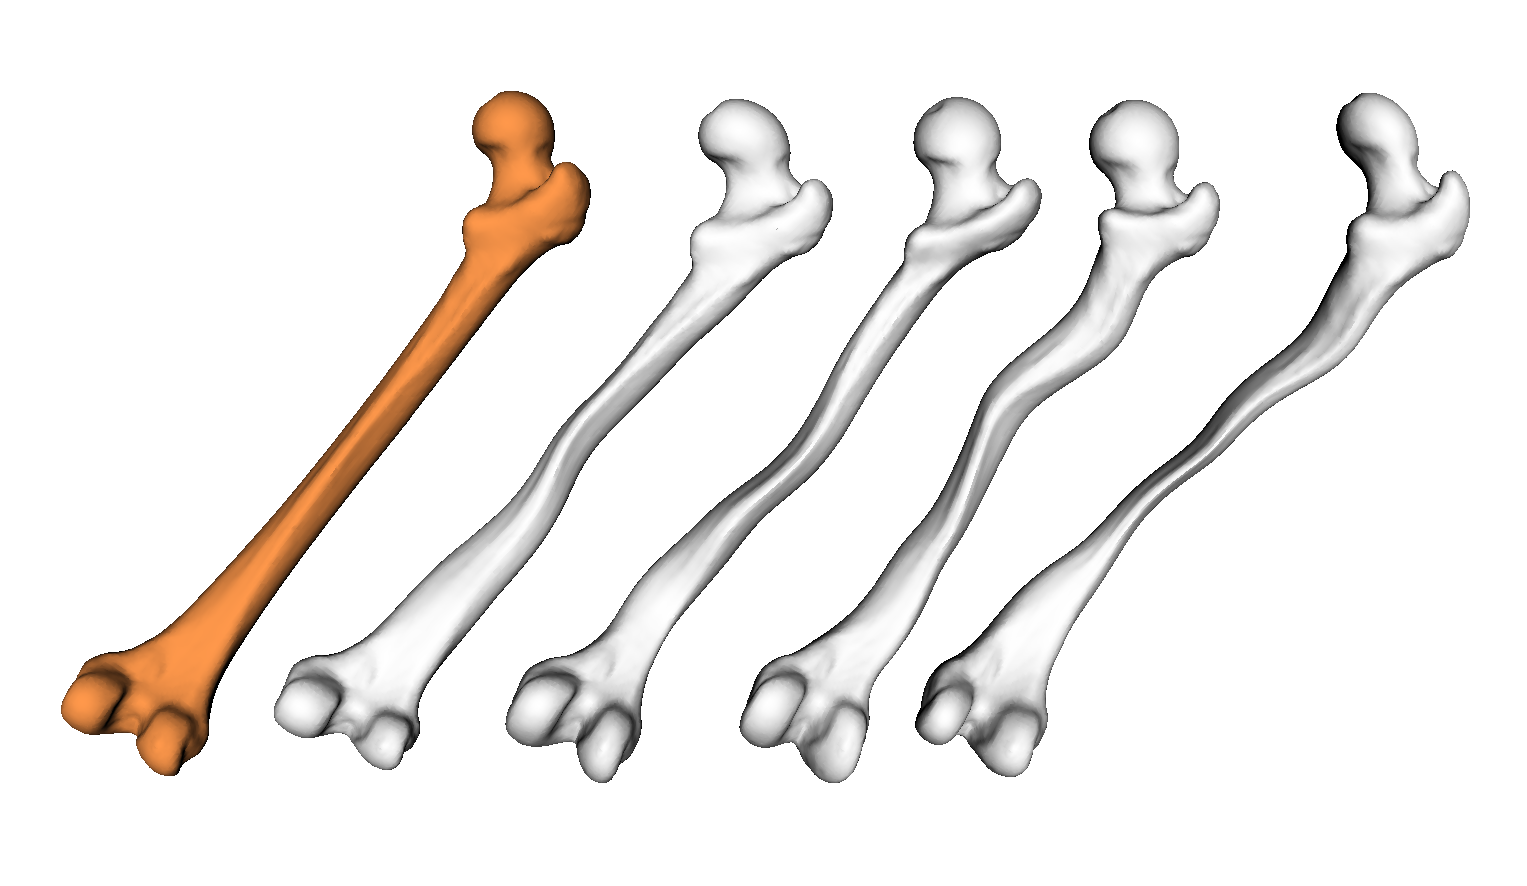
\includegraphics[width=\columnwidth]{./Figures/kernel_model_samples}
  \caption{
    The mean of our kernel model shown in orange. 
    Alongside are shown some random samples of the model.}
  \label{fig:kernel_model}
\end{figure}

%% --------------------------------------------

\subsection{Registrations}
\label{subsec:registrresults}
While in the end we are only interested in the distance between our reconstruction and the ground truth, we can also use the distance metrics as an indication of how closely our kernel model fits the training data. 
We are able to calculate these values for every element in our training data.
Hopefully, a better representation of our training data also leads to a better reconstruction of the partial bones. 

We provided mean and standard deviation of these values in \autoref{tbl:registration_distance}.

\begin{table}
\centering
\caption{Distances from fitted model to training data}
\label{tbl:registration_distance}
\begin{tabular}{lrr}
\toprule
\textbf{Bones} &
Average Distance &
Hausdorff Distance \\
\midrule
Mean& 0.63 & 11.05 \\
Standard Deviation& 0.28 & 15.45 \\
\bottomrule
\end{tabular}
\end{table}

In \autoref{fig:registration_fit} you can see an example of the kernel model fitted to the training data.

\begin{figure}
	\centering
  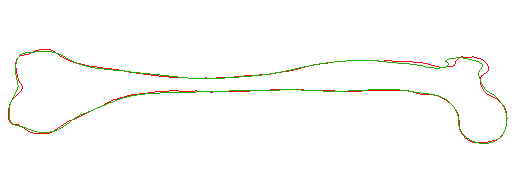
\includegraphics[scale=0.7]{./Figures/registration_fit}
  \caption{Example registration of the model to a bone from the training data}
  \label{fig:registration_fit}
\end{figure}

%% --------------------------------------------

\subsection{Trained Model}
\label{subsec:trainedmodel}
\autoref{fig:trained_model} shows the trained model we generated after fitting our kernel model to the training data.

\begin{figure}
	\centering
  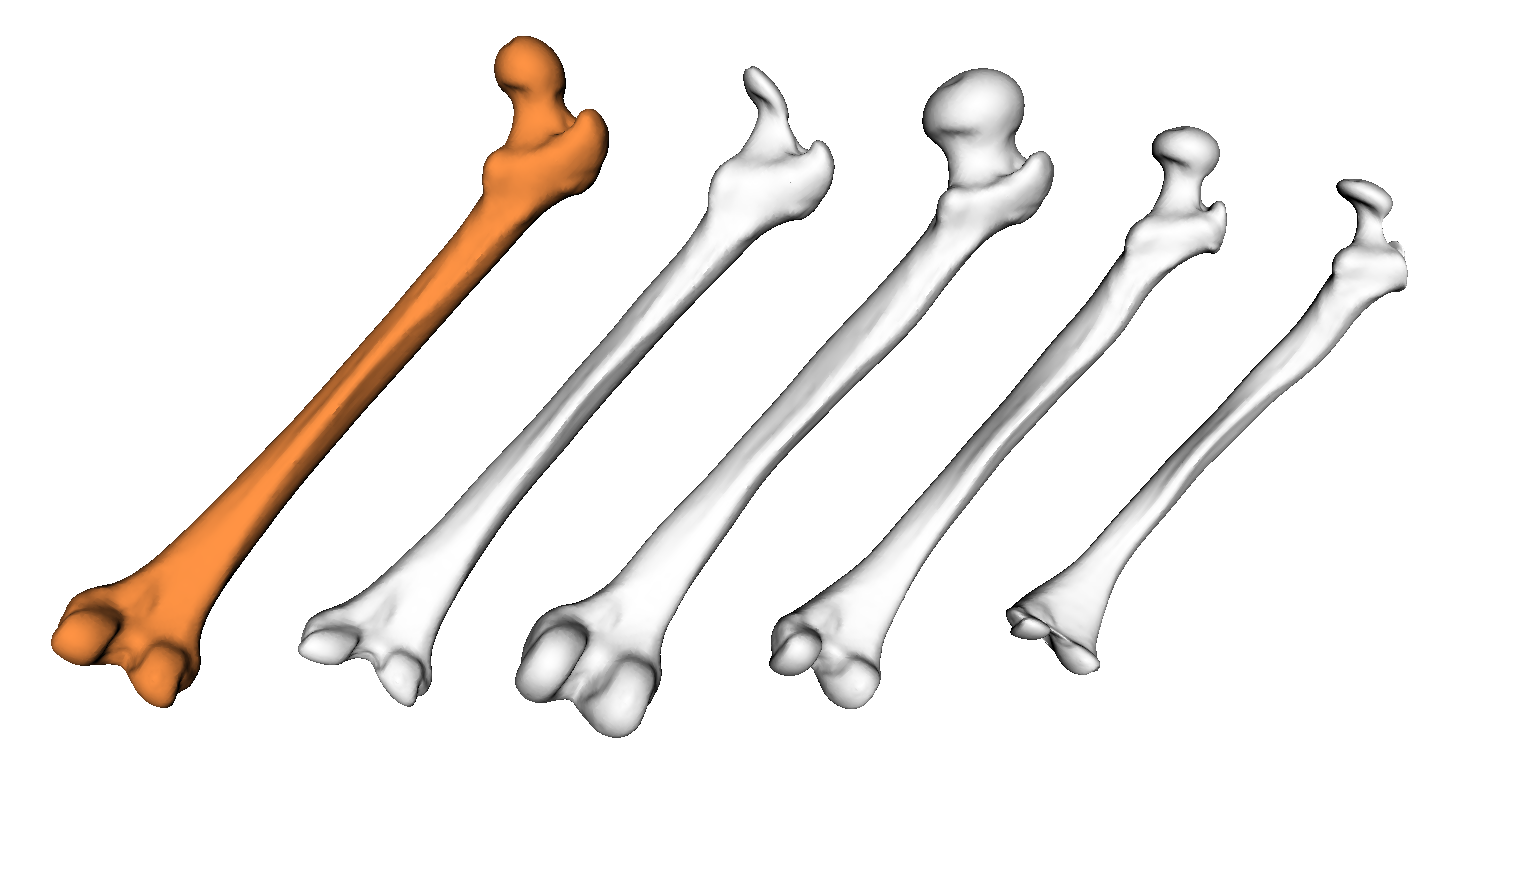
\includegraphics[width=\columnwidth]{./Figures/interpolated_model_samples}
  \caption{
    The mean of our trained model shown in orange.
    Alongside are shown some random samples of the model.}
  \label{fig:trained_model}
\end{figure}

%% --------------------------------------------

\subsection{Reconstruction of Partial Bones}
\label{subsec:reconresults}
For the evaluation of the reconstruction of the partial bones, we are interested in closely modelling the actual bone, meaning we want our reconstruction and the ground truth data (not given to us) to be as close as possible. 
This will be tested using both the average distance and the Hausdorff distance between both meshes, both of which should ideally be as small as possible.

\autoref{fig:reconstructed_bone} shows a partial bone next to its reconstruction.

\begin{figure*}
	\centering
  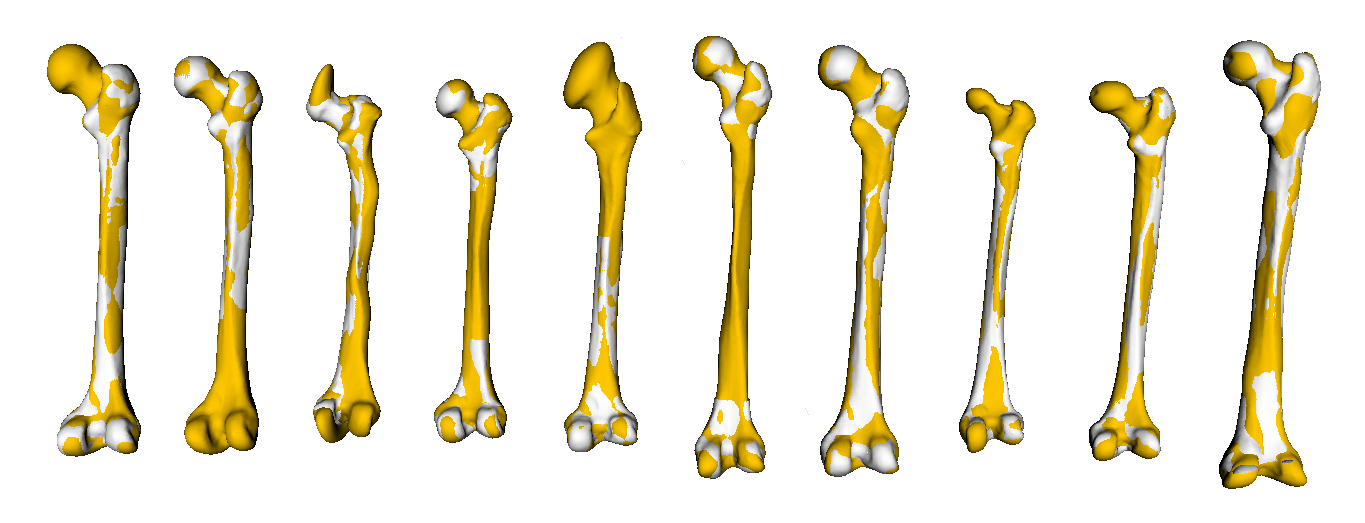
\includegraphics[width=0.82\textwidth]{./Figures/reconstruction_summary}
  \caption{All partial femurs displayed in white, aligned with our reconstruction, displayed in yellow.}
  \label{fig:reconstructed_bone}
\end{figure*}

All ten images of the partial femur bones that were given alongside our reconstruction can be found in the appendix. 
Their average distance and Hausdorff distance scores can be found in \autoref{tbl:reconstructed_distance}.

\begin{table}
\centering
\caption{Distances from reconstructed bone to ground truth.}
\label{tbl:reconstructed_distance}
\begin{tabular}{lrr}
\toprule
\textbf{Bones} &
Average Distance &
Hausdorff Distance \\
\midrule
Bone 1& 0.3 & 2 \\
Bone 2& 0.3 & 2 \\
Bone 3& 0.3 & 2 \\
Bone 4& 0.3 & 2 \\
Bone 5& 0.3 & 2 \\
Bone 6& 0.3 & 2 \\
Bone 7& 0.3 & 2 \\
Bone 8& 0.3 & 2 \\
Bone 9& 0.3 & 2 \\
Bone 10& 0.3 & 2 \\
\bottomrule
\end{tabular}
\end{table}